\documentclass[11pt]{article}

% --- PACKAGES ---
\usepackage[margin=1in]{geometry} % Set page margins
\usepackage{amsmath}             % For mathematical environments (good practice)
\usepackage{graphicx}            % To include figures later if needed
\usepackage[utf8]{inputenc}      % Input encoding
\usepackage[T1]{fontenc}         % Font encoding
\usepackage{hyperref}            % For clickable links (URLs, references)
\hypersetup{
    colorlinks=true,
    linkcolor=blue,
    filecolor=magenta,      
    urlcolor=cyan,
    pdftitle={Lala Protocol Whitepaper},
    pdfpagemode=FullScreen,
}
\usepackage{times} % Use Times font for a classic paper look (optional)
\usepackage{parskip} % Adds space between paragraphs instead of indenting (optional style choice)

% TikZ packages
\usepackage{tikz}
\usetikzlibrary{shapes.geometric, arrows.meta, positioning, chains, decorations.pathreplacing} 

% --- TIKZ STYLES ---
\tikzstyle{block} = [rectangle, draw, thick, text centered, rounded corners, minimum height=2.5em, minimum width=6em, text width=6em]
\tikzstyle{data} = [trapezium, draw, thick, text centered, rounded corners, minimum height=2.5em, text width=5em, trapezium left angle=70, trapezium right angle=110] % For data representation
\tikzstyle{decision} = [diamond, draw, thick, text centered, aspect=2, minimum width=4em, inner sep=0pt]
\tikzstyle{arrow} = [thick,->,>=Stealth] % Stealth is a nice arrow head
\tikzstyle{line} = [thick,-]

% --- DOCUMENT INFORMATION ---
\title{Lala Protocol: An AI-Advised Framework for Adaptive Blockchain}
\author{Erick Mafole\\
\texttt{erick.e.mafole@gmail.com}}
\date{\today}

% --- BEGIN DOCUMENT ---
\begin{document}

\maketitle

% --- ABSTRACT ---
\begin{abstract}
Blockchain protocols traditionally operate with static parameters, limiting their ability to efficiently adapt to dynamic network conditions and user demand. This rigidity can result in suboptimal throughput, volatile transaction fees, and delayed responses to evolving network states. Lala Protocol introduces a novel framework integrating a Proof-of-Stake (PoS) consensus layer with an \textbf{AI Advisory Module} and an on-chain \textbf{Governance Layer}. By analyzing verifiable, real-time on-chain data, the AI Advisory Module proposes adjustments to key protocol parameters. These proposals are subsequently subjected to ratification by the network's stake-weighted validators via the Governance Layer. This mechanism enables Lala Protocol to dynamically tune its operational characteristics, seeking continuous optimization for objectives such as network efficiency, economic stability, and robust security, while ensuring changes remain under decentralized control.
\end{abstract}

% --- SECTIONS ---
\section{Introduction}

\subsection{The Limitations of Static Parameters}
Existing blockchain networks often deploy with fixed operational parameters (e.g., target block time, block size limits, fee mechanism constants). While suitable for initial conditions, these static configurations inherently struggle to maintain optimal performance across the wide spectrum of real-world network dynamics. Periods of high demand can lead to severe congestion and prohibitive fees, while periods of low activity result in inefficient resource underutilization. Furthermore, adapting these parameters typically requires cumbersome off-chain coordination and manual hard-fork implementations, resulting in significant lag between observing suboptimal conditions and deploying corrective measures. This inherent inertia hinders a network's ability to reach its full potential efficiency and responsiveness.

\subsection{Lala Protocol: Enabling Governed Adaptation}
Lala Protocol addresses these limitations by introducing an automated, yet governed, adaptation layer. It leverages a standard Proof-of-Stake consensus engine for block production and finality but enhances it with two core components: an \textbf{AI Advisory Module} for intelligent analysis and a deterministic \textbf{Governance Layer} for decentralized decision-making. The protocol continuously monitors its own performance via on-chain telemetry. The AI Advisory Module analyzes this data against protocol-defined objectives and formulates specific parameter adjustment proposals. Crucially, these proposals are mere recommendations until formally ratified by the network's validators through a transparent, stake-weighted, on-chain voting process. Lala Protocol thus aims to achieve a state of continuous, dynamic optimization guided by data-driven insights but ultimately controlled by decentralized consensus.

\section{Architecture}
Lala Protocol's architecture comprises four interconnected layers (see Figure~\ref{fig:architecture}):

\begin{itemize}
    \item \textbf{2.1. Base Consensus Layer (Proof-of-Stake):} A foundational PoS engine providing Sybil resistance, block finality, and transaction ordering. Validators are selected based on staked collateral and execute the core consensus logic. This layer's state immutably stores the \textit{currently active} values of all tunable protocol parameters, ensuring network-wide agreement on operational rules.
    
    \item \textbf{2.2. Network Telemetry Module:} An integrated component within the node software responsible for deterministically calculating and aggregating key performance indicators (KPIs) from validated, on-chain data at regular intervals (e.g., per epoch). This module provides verifiable inputs for the AI Advisor. Initial KPIs include:
        \begin{itemize}
            \item Epoch Average Block Time \& Variance
            \item Epoch Average Block Resource Utilization (e.g., Gas Used / Gas Limit)
            \item Epoch Average Transaction Fee Metrics (Base Fee, Priority Fee)
            \item Validator Set Size \& Total Staked Ratio
            \item Mempool Size Trend
            \item Recent Slashing Event Count
        \end{itemize}
        
    \item \textbf{2.3. AI Advisory Module:} This module processes the aggregated data from the Telemetry Module according to predefined objective functions embedded within the protocol's specification. Its responsibilities include:
        \begin{itemize}
            \item \textit{Analysis:} Evaluating current network KPIs against target ranges or optimization goals (e.g., minimize fee volatility while maximizing throughput).
            \item \textit{Decision Logic:} Utilizing specified algorithms (initially potentially rule-based, extensible to machine learning models) to determine if parameter adjustments could better achieve the objective function(s).
            \item \textit{Proposal Formulation:} Generating cryptographically signed, standardized data structures representing proposed parameter changes (parameter identifier, current value, proposed value, target activation epoch).
            \item \textit{Deployment Note:} While the logic is protocol-defined, the execution might initially occur off-chain by whitelisted entities submitting proposals, with future research targeting verifiable, deterministic on-chain execution.
        \end{itemize}
        
    \item \textbf{2.4. Governance Layer:} An on-chain system managing the lifecycle of parameter change proposals:
        \begin{itemize}
            \item \textit{Proposal Registration:} A dedicated transaction type allows valid proposals from the AI Advisory Module (or authorized sources) to be registered on-chain.
            \item \textit{Voting Epoch:} A defined period during which active validators cast stake-weighted votes (Approve/Reject) via specific voting transactions.
            \item \textit{Threshold Validation:} Pre-defined quorum (minimum \% of total stake voting) and approval (minimum \% of voting stake approving) thresholds are checked deterministically at the end of the voting epoch.
            \item \textit{Outcome Recording:} The final ratified status (Passed/Failed) and, if passed, the activation epoch are immutably recorded in the blockchain state.
        \end{itemize}
\end{itemize}

% --- REFINED ARCHITECTURE DIAGRAM (v3 - Matching Target Image) ---
\begin{figure}[htbp] 
    \centering
    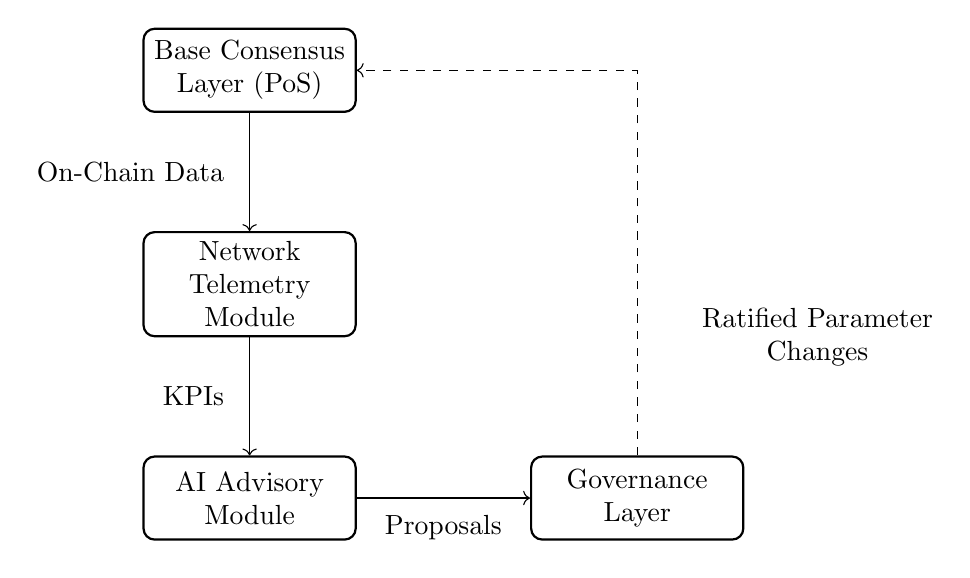
\begin{tikzpicture}[node distance=1.5cm and 2.2cm] 
        
        \tikzstyle{block} = [rectangle, draw, thick, text centered, rounded corners, minimum height=3em, minimum width=7em, text width=7em, align=center] 
        
        \node (base) [block] {Base Consensus Layer (PoS)};
        \node (telemetry) [block, below=of base] {Network Telemetry Module};
        \node (ai) [block, below=of telemetry, node distance=1.8cm] {AI Advisory Module};
        \node (gov) [block, right=of ai] {Governance Layer}; 
        
        % Solid arrows
        \draw [->] (base.south) -- node[midway, left=0.2cm] {On-Chain Data} (telemetry.north);
        \draw [->] (telemetry.south) -- node[midway, left=0.2cm] {KPIs} (ai.north);
        \draw [->] (ai.east) -- node[midway, below=0.1cm] {Proposals} (gov.west);

        % Feedback loop (dotted line)
        \coordinate (gov_top) at ([yshift=1.5cm]gov.north); % Reduced height
        \coordinate (base_corner) at (base.east -| gov_top); % Aligned with base's center
        
        % Dotted line path
        \draw [->, dashed] (gov.north) -- (gov_top) -- (base_corner) -- (base.east);
        
        % Label positioned beside the horizontal segment of the dotted line
        \node [right=0.2cm, align=center] at ([xshift=0.5cm]gov_top -| base_corner) {Ratified Parameter\\Changes};

    \end{tikzpicture}
    \caption{High-Level Architecture of Lala Protocol} 
    \label{fig:architecture} 
\end{figure}

\section{Core Mechanisms}
The interaction between the layers follows a defined process:

\begin{itemize}
    \item \textbf{3.1. Deterministic Data Aggregation:} Nodes compute telemetry KPIs based solely on finalized block data from preceding epochs, ensuring all nodes derive identical inputs for potential AI analysis or governance verification.
    
    \item \textbf{3.2. AI Analysis \& Proposal Generation:} The AI module reads the latest epoch's telemetry data from the state. Based on its internal logic and objective functions (e.g., "IF \texttt{avg\_block\_utilization} < 40\% for 3 epochs AND \texttt{avg\_tx\_fee} < \texttt{min\_fee\_target} THEN propose increasing \texttt{block\_gas\_limit} by 5\%"), it may generate a signed proposal structure.
    
    \item \textbf{3.3. Proposal Ratification \& Voting:} Validators identify active proposals in the state, evaluate them (potentially using their own off-chain analysis), and submit vote transactions referencing the proposal ID. At the end of the voting epoch, nodes deterministically tally votes based on validator stake recorded at the epoch's start.
    
    \item \textbf{3.4. Synchronized Parameter Activation:} If a proposal is ratified, the node's state transition function includes logic to check the current epoch number against the activation epoch stored in the passed proposal's outcome. Precisely at the beginning of the activation epoch, all nodes switch to using the newly ratified parameter value for all subsequent consensus calculations, maintaining network coherency. This adaptation process follows a specific loop, illustrated in Figure~\ref{fig:adaptation_loop}.
\end{itemize}

\begin{figure}[htbp]
    \centering
    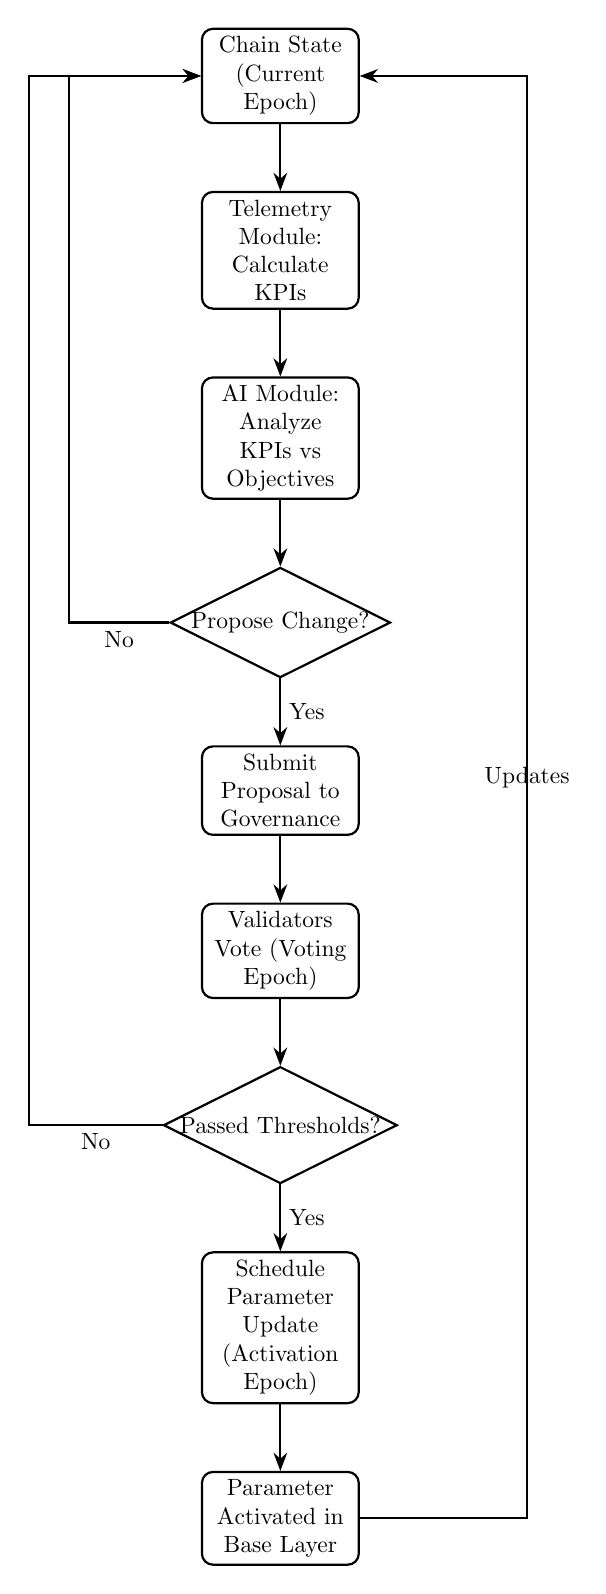
\begin{tikzpicture}[node distance=1cm and 1.5cm, >=Stealth, start chain=going below, scale=0.85, transform shape] % Added scaling to fit page
        
        % Nodes using chain library for easier vertical layout
        \node (start) [block, on chain] {Chain State (Current Epoch)};
        \node (telemetry) [block, on chain] {Telemetry Module: Calculate KPIs};
        \node (ai) [block, on chain] {AI Module: Analyze KPIs vs Objectives};
        \node (dec_propose) [decision, on chain, node distance=1.5cm] {Propose Change?}; % Increased distance for clarity
        \node (submit) [block, on chain, node distance=1.5cm] {Submit Proposal to Governance};
        \node (vote) [block, on chain] {Validators Vote (Voting Epoch)};
        \node (dec_passed) [decision, on chain, node distance=1.5cm] {Passed Thresholds?};
        \node (schedule) [block, on chain, node distance=1.5cm] {Schedule Parameter Update (Activation Epoch)};
        \node (activate) [block, on chain] {Parameter Activated in Base Layer};
        
        % Arrows for the main flow
        \draw [arrow] (start) -- (telemetry);
        \draw [arrow] (telemetry) -- (ai);
        \draw [arrow] (ai) -- (dec_propose);
        \draw [arrow] (dec_propose) -- node[midway, right] {Yes} (submit);
        \draw [arrow] (submit) -- (vote);
        \draw [arrow] (vote) -- (dec_passed);
        \draw [arrow] (dec_passed) -- node[midway, right] {Yes} (schedule);
        \draw [arrow] (schedule) -- (activate);
        
        % Loop back arrow (can be tricky, adjust coordinates as needed)
        \draw [arrow] (activate.east) -- ++(2.5cm,0) |- node[pos=0.25, above] {Updates} (start.east); 
        
        % 'No' branches from decisions
        \draw [arrow] (dec_propose.west) -- ++(-1.5cm,0) node[midway, below] {No} |- (start.west); % Loop back if no proposal
        \draw [arrow] (dec_passed.west) -- ++(-2cm,0) node[midway, below] {No} |- (start.west); % Loop back if proposal fails
        
    \end{tikzpicture}
    \caption{Lala Protocol Parameter Adaptation Loop}
    \label{fig:adaptation_loop}
\end{figure}

\clearpage

\section{Economic Alignment \& Incentives}
Lala Protocol utilizes standard PoS incentives (block rewards, transaction fees) to secure the network. The adaptive mechanism aims to enhance these incentives by fostering a healthier, more predictable network environment. By mitigating extreme fee spikes or network stalls, it seeks to improve the user experience and potentially increase overall network value, indirectly benefiting validators. The mechanism directly influences the fee market and block space allocation dynamics. The governance component further aligns validators by giving them direct control over the evolution of the protocol's operational parameters based on AI-driven recommendations.

\section{Future Research \& Considerations}
\begin{itemize}
    \item \textbf{AI Model Sophistication:} Exploring advanced, potentially more predictive ML models (e.g., Reinforcement Learning) for the Advisory Module, while addressing verifiability.
    \item \textbf{Objective Function Design:} Formalizing robust and potentially multi-objective optimization goals that capture desired network states without introducing instability.
    \item \textbf{Formal Verification \& Stability Analysis:} Rigorously modeling the feedback loop between parameter changes and network behavior to prove stability and prevent unintended oscillations or exploits.
    \item \textbf{Governance Robustness:} Analyzing voter behavior, potential apathy, and mechanisms to incentivize informed participation in parameter governance.
    \item \textbf{External Data Integration:} Investigating secure and decentralized oracle solutions if off-chain data becomes necessary for more complex objective functions.
    \item \textbf{Ecosystem Tooling:} Developing explorers and wallets that clearly visualize parameter history, active proposals, and voting participation.
\end{itemize}

\section{Conclusion}
Lala Protocol proposes a significant step beyond statically configured blockchains by introducing a mechanism for intelligent, governed adaptation. By combining AI-driven analysis of on-chain data with a robust PoS-based governance framework, the protocol aims to continuously tune its parameters for optimal performance, stability, and efficiency. This adaptive capability promises a more resilient and responsive network, capable of navigating dynamic conditions while upholding the core principles of decentralized control and consensus.

\vspace{0.5cm} % Add some vertical space to separate the quote
\noindent \textit{"Either I'm crazy or I don't know what I'm doing. Which simply means I am crazy recursively." - Erick Mafole}
% Remove the \bibdata command that's causing the error
% \bibdata{simple}

% --- END DOCUMENT ---
\end{document}